\section{Method}
\subsection{Overview}

Given a triangle mesh and a set of posed reference images, we bake the object's appearance into a field that a rasterizer can evaluate per fragment in real time. The mesh is fixed; only the appearance on it is optimized. Sec.~\ref{sec:downstream} then describes two downstream tasks the baked asset supports, neither of
which alters the pipeline above.

We bake appearance with three interchangeable modules and composite their outputs at each fragment.
An on-manifold 2D Gaussian mixture (Sec.~\ref{sec:gmm}) carries the view-independent fields; an
adaptive environment map (Sec.~\ref{sec:env}) supplies the incident radiance, including the light
the object casts on itself; and a compact FastKAN decoder (Sec.~\ref{sec:kan}) turns a lookup into
that map into a view-dependent reflection. At a visible surface point $\mathbf{x}$ seen along view
direction $\mathbf{v}$, the three combine as
%
\begin{equation}
c(\mathbf{x}, \mathbf{v}) = \operatorname{sigmoid}\!\Big( \operatorname{logit}\big(a(\mathbf{x})\big)
+ m(\mathbf{x})\, r(\mathbf{x}, \mathbf{v}) \Big),
\label{eq:appearance}
\end{equation}
%
where the albedo $a(\mathbf{x})\in[0,1]^3$ and the reflectivity $m(\mathbf{x})\in[0,1]$ are read
from the mixture ($m{=}0$ matte, $m{=}1$ mirror) and the residual $r(\mathbf{x},\mathbf{v})$ is
emitted by the decoder. Compositing in logit space lets the reflection act as an additive residual
on the diffuse base while keeping the result in $[0,1]$ without clamping; $m$ gates where it
applies. 

\subsection{2D Gaussian Mixture on the Manifold}
\label{sec:gmm}
The albedo and reflectivity fields are stored by a mixture of $N$ two-dimensional Gaussian
``disks'' on the mesh surface ($N{=}10^6$ in our experiments). $N$ is fixed at initialization and
never changes during training: there is no densification, pruning, or opacity culling. The count can
be reduced after training, without retraining, by the compaction of Sec.~\ref{sec:Compaction}.

\paragraph{On-manifold anchoring.}
Each disk $i$ is assigned to a single triangle $f_i$ and a barycentric coordinate
$\mathbf{b}_i=(b_{i,0},b_{i,1},b_{i,2})$ with $b_{i,k}\ge 0$ and $\sum_k b_{i,k}=1$.
Its center is \emph{reconstructed} from the live vertices of that triangle,
%
\begin{equation}
\mathbf{x}_i = b_{i,0}\,\mathbf{p}_0(f_i) + b_{i,1}\,\mathbf{p}_1(f_i) + b_{i,2}\,\mathbf{p}_2(f_i),
\label{eq:center}
\end{equation}
%
so $\mathbf{x}_i$ is by construction a convex combination of the face's vertices and lies exactly on
the triangle. The face therefore supplies the disk's frame as well as its position: its extent lives
in the in-plane axes $(\mathbf{t}_1,\mathbf{t}_2)$ of $f_i$, with an in-plane rotation $\theta_i$
about the face normal $\mathbf{n}$ and an anisotropic in-plane scale $(s_{i,1},s_{i,2})$. We give
the disk \emph{no extent along} $\mathbf{n}$, so it is a strictly two-dimensional element rather
than a three-dimensional one with a constrained center.

\paragraph{Per-disk attributes.}
Each disk carries two view-independent attributes: an albedo $a_i\in[0,1]^3$ and a scalar reflectivity $m_i\in[0,1]$, both stored as unconstrained logits and squashed at use.
The continuous fields $a(\mathbf{x})$ and $m(\mathbf{x})$ in Eq.~\eqref{eq:appearance} are obtained by blending these per-disk attributes over the disks near $\mathbf{x}$ (described next).

\paragraph{Partition-of-unity blend.}
A fragment at $\mathbf{x}$ on face $f$ gathers from $\mathcal{N}(f)$, the fixed set of the $K{=}16$ disks nearest that face. These disks are not restricted to $f$: the top-$K$ set spans $f$ and its neighboring faces, so the gather crosses face boundaries rather than being truncated per face. Each disk is weighted by its own Gaussian density at $\mathbf{x}$, evaluated in the disk's tangent frame:
\begin{equation}
w_k(\mathbf{x}) = \exp\!\Big(-\tfrac12\big[(u_{k,1}/s_{k,1})^2 + (u_{k,2}/s_{k,2})^2\big]\Big), \quad
\bar{w}_k(\mathbf{x}) = w_k(\mathbf{x}) \Big/ \sum_{j\in\mathcal{N}(f)} w_j(\mathbf{x}),
\label{eq:pou}
\end{equation}
where $u_{k,j}=(\mathbf{x}-\mathbf{x}_k)\cdot\mathbf{t}_{k,j}$ is the fragment's in-plane offset from disk $k$'s center along its tangent axis $\mathbf{t}_{k,j}$. The per-fragment fields are the resulting convex combination,
\begin{equation}
a(\mathbf{x}) = \sum_{k\in\mathcal{N}(f)} \bar{w}_k(\mathbf{x})\, a_k,  \quad
m(\mathbf{x}) = \operatorname{sigmoid}\!\Big(\sum_{k\in\mathcal{N}(f)} \bar{w}_k(\mathbf{x})\, \operatorname{logit}(m_k)\Big),
\label{eq:blend}
\end{equation}
with $a_k,m_k$ the squashed per-disk albedo and reflectivity. The weights form a partition of unity
($\sum_k \bar{w}_k = 1$), so each field is a \emph{normalized} convex combination of the nearby
disks rather than an alpha composite. This is the order-independence the representation was designed
around (Sec.~\ref{sec:intro}): the blend never asks which disk lies in front, so the coplanar depth
ties cannot arise and the $\mathcal{O}(K)$ gather needs no sort.

\subsection{Adaptive Environment Map}
\label{sec:env}
We describe the reflection lookup first without its learned parts, where it is ordinary environment mapping: a directional fetch and a weighted blend.

\paragraph{Fetching}
Treat the environment as a classical equirectangular map. At a surface point with normal $\mathbf{n}$ seen from view direction $\mathbf{v}$, the mirror-reflected direction is $\boldsymbol{\omega}_r = 2(\mathbf{n}\cdot\mathbf{v})\,\mathbf{n} - \mathbf{v}$. We then start a longitude--elevation coordinate and bilinearly sample according to the direction.

\paragraph{Which map: near-convex parts.}
A single global map assumes all light arrives from infinitely far away, so it cannot reproduce the
light an object casts on itself. We resolve this geometrically. Within a convex part there is no
self-occlusion and no self-reflection, so all incident light is external and a single directional
map is a good approximation; what a global map cannot capture is the light exchanged \emph{between}
parts. We therefore split the object into near-convex parts with a convex
decomposition~\citep{coacd} and give each part its own map, so that light reaching a part from the
rest of the object is absorbed into that part's map and read back as an ordinary far-field lookup.
The approximation is that this inter-part light is treated as distant and position-independent
within a part, and
Sec.~\ref{sec:ablation} measures what it recovers.
\begin{figure}[t]
    \centering
    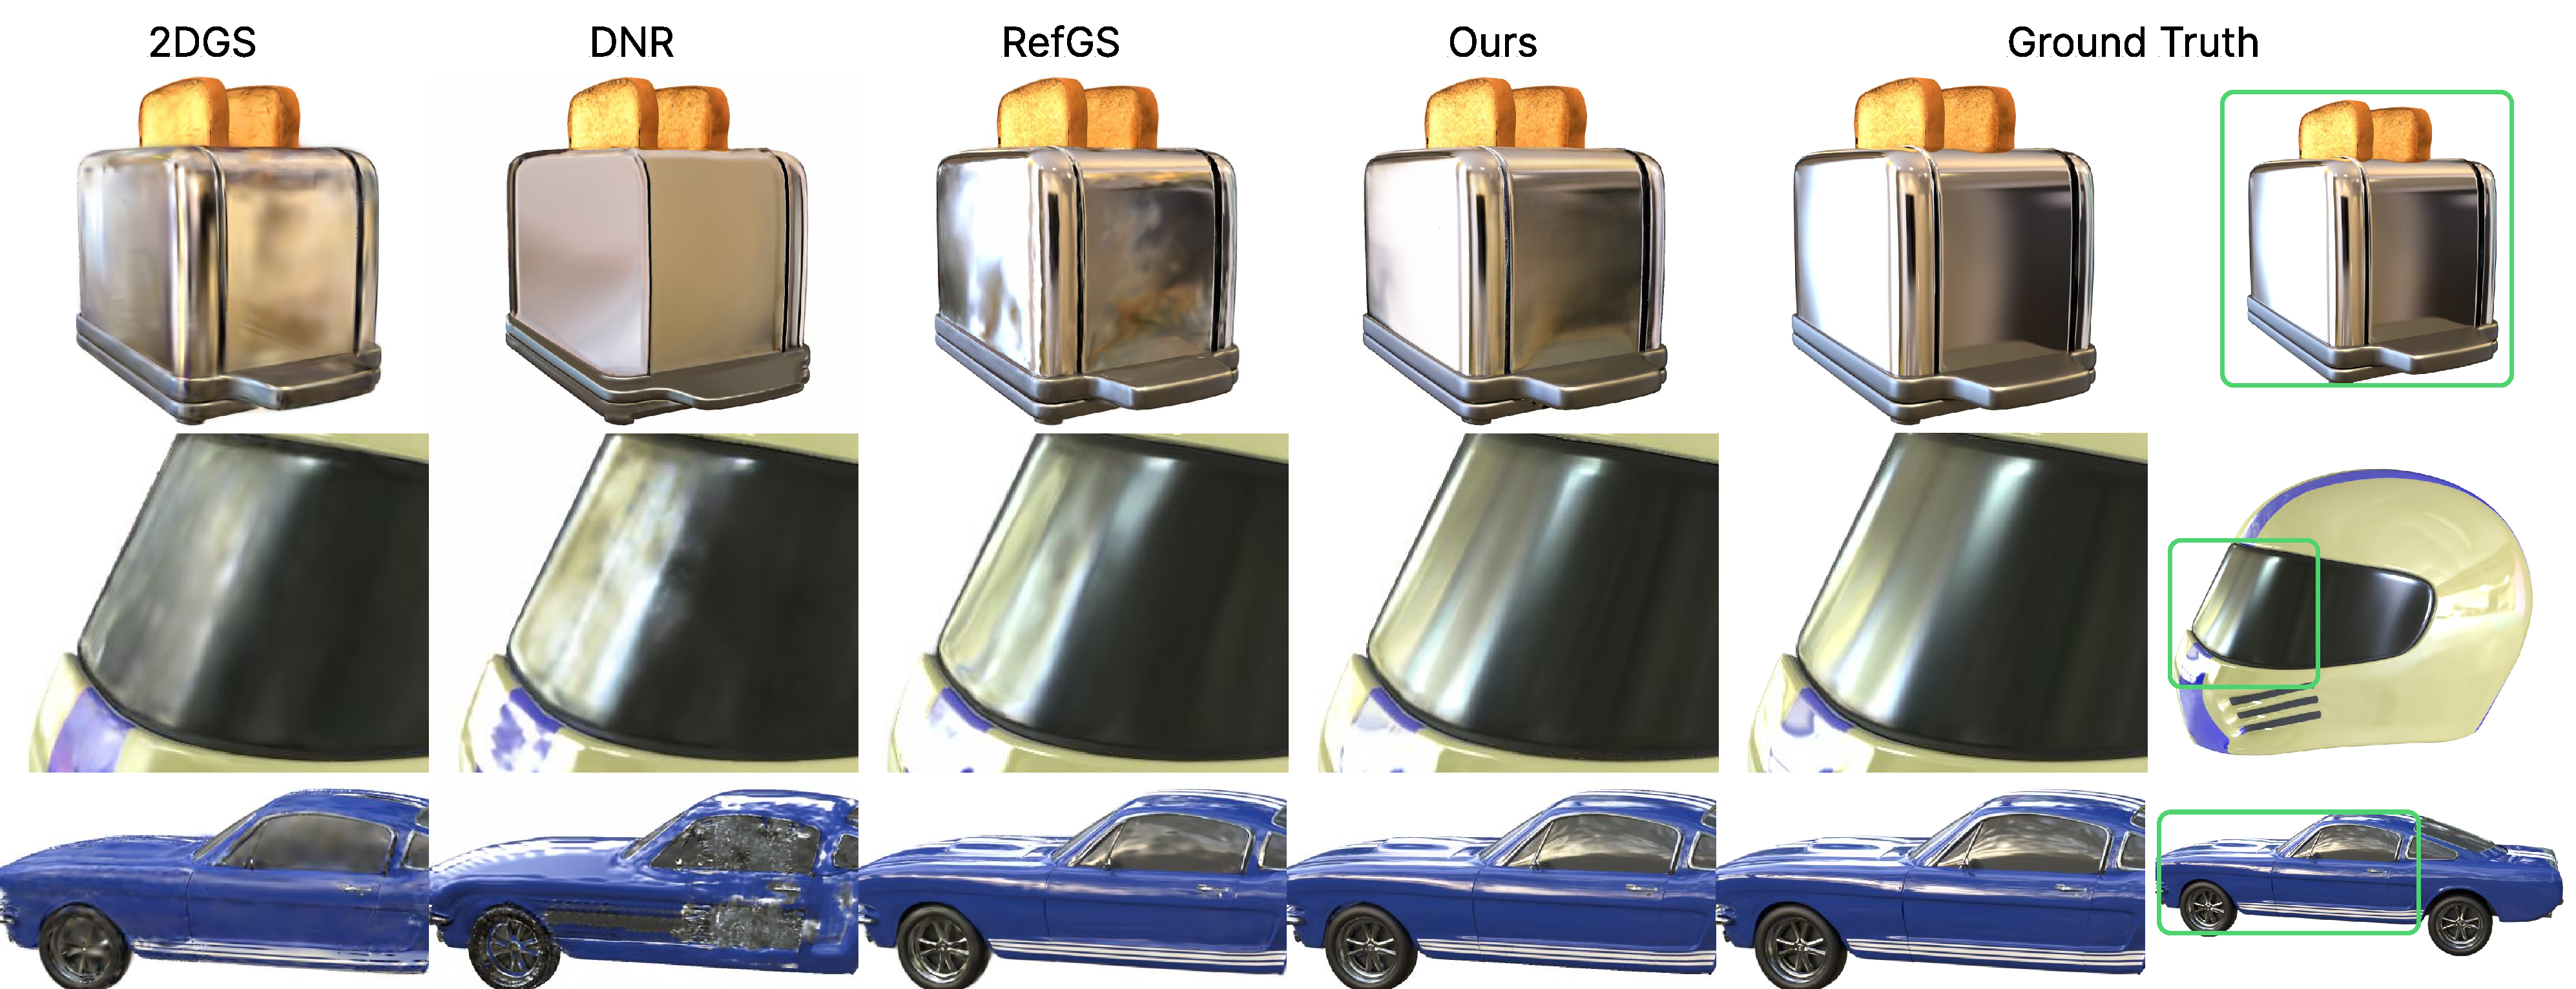
\includegraphics[width=0.95\linewidth]{figs/qualitative.pdf}
    \caption{\textbf{Qualitative comparison on Shiny-Blender.} From left to right: the mesh-constrained baseline 2DGS$^{*}$, DNR, the state-of-the-art RefGS, our method, and ground truth (GT). Our renders reproduce the sharp, high-frequency environment reflections on the metallic surfaces most faithfully; 2DGS$^{*}$ and DNR blur or smear them, RefGS recovers them less crisply.}
    \label{fig:qualitative}
    \vspace{-2mm}
\end{figure}
\paragraph{Growing the maps by error.}
We do not fix the number of maps in advance. Training begins with one map shared by the whole object. Periodically we attribute the current reconstruction error to parts and split off the highest-error \emph{connected} region into a new child map, warm-started by copying its parent. Repeated up to a small budget (five maps in our experiments), this spends capacity where reflection error is largest, isolating the concave pockets a single map cannot explain.

\paragraph{Blending across borders.}
Hard per-face routing would leave visible seams at part boundaries. Instead, each face holds a soft
membership over the maps and a fragment reads \emph{every} map at $\boldsymbol{\omega}_r$:
%
\begin{equation}
E(\boldsymbol{\omega}_r, f) = \sum_{p} \beta_p(f)\, E_p(\boldsymbol{\omega}_r),
\qquad
\beta_p(f) = \operatorname{softmax}_p\!\big(-d_p(f)/\tau\big),
\label{eq:envblend}
\end{equation}
%
where $d_p(f)$ is the distance from face $f$ to the nearest face assigned to map $p$, and $\tau$
sets the blend width: $\beta$ is $\approx$ one-hot inside a region and blends smoothly within
$\sim\tau$ of a border, so the weighted fetch removes the seam. Each $E_p$ stores a learned
multi-channel feature rather than RGB, decoded into reflected color by the network of
Sec.~\ref{sec:kan}.

\subsection{The FastKAN Reflection Decoder}
\label{sec:kan}
The fields of Secs.~\ref{sec:gmm} and~\ref{sec:env} are tied together by a learnable decoder: it
consumes a surface point, its viewing geometry, and the part-blended environment feature, and emits
the view-dependent reflection $r(\mathbf{x},\mathbf{v})$ of Eq.~\eqref{eq:appearance}. The decoder
is interchangeable. We use a Fast Kolmogorov--Arnold Network, which places a learnable activation on
every \emph{edge} rather than a fixed nonlinearity on every node \cite{kan}, realized with Gaussian
radial basis functions on a small fixed grid \cite{fastkan}; on our task it outperforms a
parameter-matched MLP by $1.39$ dB (Sec.~\ref{sec:ablation}). Where inference cost matters more than
fidelity, an MLP or a precomputed lookup table can occupy the same slot.

\paragraph{Staged inputs.}
The decoder is a deferred, staged shader~\citep{refnerf}: view-independent quantities are consumed
before view-dependent ones, with two KAN layers per stage. (1) \emph{Position}: the Fourier
positional encoding of the hit point $\mathbf{x}$ (bounding-box normalized, six frequencies), which
localizes appearance on the surface. (2) \emph{Normal}: the real spherical harmonics
$\mathrm{SH}(\mathbf{n})$ of the surface normal (degree $4$) are appended. (3) \emph{View}: the
integrated directional encoding $\mathrm{IDE}(\boldsymbol{\omega}_r)$ of the reflected direction is
appended together with $\mathbf{n}\!\cdot\!\mathbf{v}$; the IDE is $\mathrm{SH}(\boldsymbol{\omega}_r)$
attenuated by a learned per-point roughness, so a rougher surface queries the environment over a
wider cone --- a prefiltered, glossy lookup rather than a perfect mirror. This stage emits the
material feature $\mathbf{h}$.

\paragraph{Environment fusion and output.}
A two-layer linear MLP fuses $\mathbf{h}$ with the part-blended environment feature
$E(\boldsymbol{\omega}_r,f)$ of Eq.~\eqref{eq:envblend}, and a linear head emits the reflection
$r(\mathbf{x},\mathbf{v})$ of Eq.~\eqref{eq:appearance}, scaled by a learned specular tint in
$[0,1]^3$. Only the staged trunk is KAN. The color head is zero-initialized, so reflection starts at
zero and is turned \emph{up} only where the training views demand it.

\subsection{Downstream Tasks}
\label{sec:downstream}
The baked asset supports two tasks beyond rendering. Both operate on a trained model and leave the
representation of Secs.~\ref{sec:gmm}--\ref{sec:kan} unchanged.
\subsubsection{Mesh Refinement}
\label{sec:refinement}
Anchoring leaves the field blind along the surface normal: the blend weights of Eq.~\eqref{eq:pou}
depend only on in-plane offsets, so a gradient evaluated on the surface vanishes in $\mathbf{n}$. A
disk can ask the mesh to slide, never to move in or out. We recover the missing direction by
detaching the disk centers for a single backward pass and evaluating them in ray-splat
form~\citep{2DGS}, which reads where each disk would move if it were free. That request is then
distributed onto the face's vertices through the same barycentric weights that reconstructed it,
restricted to the vertex normal, band-limited to the disk radius, and capped per cycle. The disks
themselves never leave the surface: they are re-anchored once the vertex update commits, so the
field remains a parameterization of the mesh throughout. Alternating this geometry step with an
ordinary appearance step refines the mesh the asset is baked onto; we evaluate it in
Sec.~\ref{sec:Exp} and give the algorithm in \textcolor{red}{App.~\ref{app:refinement}.}
